%%
%% Automatically generated file from DocOnce source
%% (https://github.com/hplgit/doconce/)
%%

% #define PREAMBLE

% #ifdef PREAMBLE
%-------------------- begin preamble ----------------------

\documentclass[%
oneside,                 % oneside: electronic viewing, twoside: printing
final,                   % draft: marks overfull hboxes, figures with paths
10pt,french]{article}

\listfiles               %  print all files needed to compile this document

\usepackage{relsize,makeidx,color,setspace,amsmath,amsfonts,amssymb}
\usepackage[table]{xcolor}
\usepackage{bm,ltablex,microtype}

\usepackage[pdftex]{graphicx}

% Packages for typesetting blocks of computer code
\usepackage{fancyvrb,framed,moreverb}

% Define colors
\definecolor{orange}{cmyk}{0,0.4,0.8,0.2}
\definecolor{tucorange}{rgb}{1.0,0.64,0}
\definecolor{darkorange}{rgb}{.71,0.21,0.01}
\definecolor{darkgreen}{rgb}{.12,.54,.11}
\definecolor{myteal}{rgb}{.26, .44, .56}
\definecolor{gray}{gray}{0.45}
\definecolor{mediumgray}{gray}{.8}
\definecolor{lightgray}{gray}{.95}
\definecolor{brown}{rgb}{0.54,0.27,0.07}
\definecolor{purple}{rgb}{0.5,0.0,0.5}
\definecolor{darkgray}{gray}{0.25}
\definecolor{darkblue}{rgb}{0,0.08,0.45}
\definecolor{darkblue2}{rgb}{0,0,0.8}
\definecolor{lightred}{rgb}{1.0,0.39,0.28}
\definecolor{lightgreen}{rgb}{0.48,0.99,0.0}
\definecolor{lightblue}{rgb}{0.53,0.81,0.92}
\definecolor{lightblue2}{rgb}{0.3,0.3,1.0}
\definecolor{lightpurple}{rgb}{0.87,0.63,0.87}
\definecolor{lightcyan}{rgb}{0.5,1.0,0.83}

\colorlet{comment_green}{green!50!black}
\colorlet{string_red}{red!60!black}
\colorlet{keyword_pink}{magenta!70!black}
\colorlet{indendifier_green}{green!70!white}

% Backgrounds for code
\definecolor{cbg_gray}{rgb}{.95, .95, .95}
\definecolor{bar_gray}{rgb}{.92, .92, .92}

\definecolor{cbg_yellowgray}{rgb}{.95, .95, .85}
\definecolor{bar_yellowgray}{rgb}{.95, .95, .65}

\colorlet{cbg_yellow2}{yellow!10}
\colorlet{bar_yellow2}{yellow!20}

\definecolor{cbg_yellow1}{rgb}{.98, .98, 0.8}
\definecolor{bar_yellow1}{rgb}{.98, .98, 0.4}

\definecolor{cbg_red1}{rgb}{1, 0.85, 0.85}
\definecolor{bar_red1}{rgb}{1, 0.75, 0.85}

\definecolor{cbg_blue1}{rgb}{0.87843, 0.95686, 1.0}
\definecolor{bar_blue1}{rgb}{0.7,     0.95686, 1}

%\setlength{\fboxsep}{-1.5mm}  % adjust cod_vpad/pro_vpad background box

%% Background for code blocks (parameter is color name)

%% pro/cod_vpad: gives some vertical padding before and after the text
%% (but has more simplistic code than _cod/pro_tight+cod/pro).
%% pro/cod_vpad can be used to enclose Verbatim or lst begin/end for code.
%% pro/cod calls _pro/cod_tight and has very little vertical padding,
%% used to enclose Verbatim and other begin/end for code.
%% (pro/cod is what the ptex2tex program could produce with the
%% Blue/BlueBar definitions in .ptex2tex.cfg.)

\newenvironment{cod_vpad}[1]{
   \def\FrameCommand{\colorbox{#1}}
   \MakeFramed{\FrameRestore}}
   {\endMakeFramed}

\newenvironment{_cod_tight}[1]{
   \def\FrameCommand{\colorbox{#1}}
   \FrameRule0.6pt\MakeFramed {\FrameRestore}\vskip3mm}
   {\vskip0mm\endMakeFramed}

\newenvironment{cod}[1]{
\bgroup\rmfamily
\fboxsep=0mm\relax
\begin{_cod_tight}{#1}
\list{}{\parsep=-2mm\parskip=0mm\topsep=0pt\leftmargin=2mm
\rightmargin=2\leftmargin\leftmargin=4pt\relax}
\item\relax}
{\endlist\end{_cod_tight}\egroup}

%% Background for complete program blocks (parameter 1 is color name
%% for background, parameter 2 is color for left bar)
\newenvironment{pro_vpad}[2]{
   \def\FrameCommand{\color{#2}\vrule width 1mm\normalcolor\colorbox{#1}}
   \MakeFramed{\FrameRestore}}
   {\endMakeFramed}

\newenvironment{_pro_tight}[2]{
   \def\FrameCommand{\color{#2}\vrule width 1mm\normalcolor\colorbox{#1}}
   \FrameRule0.6pt\MakeFramed {\advance\hsize-2mm\FrameRestore}\vskip3mm}
   {\vskip0mm\endMakeFramed}

\newenvironment{pro}[2]{
\bgroup\rmfamily
\fboxsep=0mm\relax
\begin{_pro_tight}{#1}{#2}
\list{}{\parsep=-2mm\parskip=0mm\topsep=0pt\leftmargin=2mm
\rightmargin=2\leftmargin\leftmargin=4pt\relax}
\item\relax}
{\endlist\end{_pro_tight}\egroup}

\usepackage{minted}
\usemintedstyle{default}

\usepackage[T1]{fontenc}
%\usepackage[latin1]{inputenc}
\usepackage{ucs}
\usepackage[utf8x]{inputenc}

\usepackage{lmodern}         % Latin Modern fonts derived from Computer Modern

% Hyperlinks in PDF:
\definecolor{linkcolor}{rgb}{0,0,0.4}
\usepackage{hyperref}
\hypersetup{
    breaklinks=true,
    colorlinks=true,
    linkcolor=linkcolor,
    urlcolor=linkcolor,
    citecolor=black,
    filecolor=black,
    %filecolor=blue,
    pdfmenubar=true,
    pdftoolbar=true,
    bookmarksdepth=3   % Uncomment (and tweak) for PDF bookmarks with more levels than the TOC
    }
%\hyperbaseurl{}   % hyperlinks are relative to this root

\setcounter{tocdepth}{2}  % levels in table of contents

% Tricks for having figures close to where they are defined:
% 1. define less restrictive rules for where to put figures
\setcounter{topnumber}{2}
\setcounter{bottomnumber}{2}
\setcounter{totalnumber}{4}
\renewcommand{\topfraction}{0.95}
\renewcommand{\bottomfraction}{0.95}
\renewcommand{\textfraction}{0}
\renewcommand{\floatpagefraction}{0.75}
% floatpagefraction must always be less than topfraction!
% 2. ensure all figures are flushed before next section
\usepackage[section]{placeins}
% 3. enable begin{figure}[H] (often leads to ugly pagebreaks)
%\usepackage{float}\restylefloat{figure}

% --- fancyhdr package for fancy headers ---
\usepackage{fancyhdr}
\fancyhf{} % sets both header and footer to nothing
\renewcommand{\headrulewidth}{0pt}
\fancyfoot[LE,RO]{\thepage}
% Ensure copyright on titlepage (article style) and chapter pages (book style)
\fancypagestyle{plain}{
  \fancyhf{}
  \fancyfoot[C]{{\footnotesize \copyright\ 2019, Ahmed Ammar. Released under CC Attribution 4.0 license}}
%  \renewcommand{\footrulewidth}{0mm}
  \renewcommand{\headrulewidth}{0mm}
}
% Ensure copyright on titlepages with \thispagestyle{empty}
\fancypagestyle{empty}{
  \fancyhf{}
  \fancyfoot[C]{{\footnotesize \copyright\ 2019, Ahmed Ammar. Released under CC Attribution 4.0 license}}
  \renewcommand{\footrulewidth}{0mm}
  \renewcommand{\headrulewidth}{0mm}
}

\pagestyle{fancy}


% prevent orhpans and widows
\clubpenalty = 10000
\widowpenalty = 10000

\newenvironment{doconceexercise}{}{}
\newcounter{doconceexercisecounter}


% ------ header in subexercises ------
%\newcommand{\subex}[1]{\paragraph{#1}}
%\newcommand{\subex}[1]{\par\vspace{1.7mm}\noindent{\bf #1}\ \ }
\makeatletter
% 1.5ex is the spacing above the header, 0.5em the spacing after subex title
\newcommand\subex{\@startsection{paragraph}{4}{\z@}%
                  {1.5ex\@plus1ex \@minus.2ex}%
                  {-0.5em}%
                  {\normalfont\normalsize\bfseries}}
\makeatother


% --- end of standard preamble for documents ---


\usepackage[french]{babel}

% insert custom LaTeX commands...

\raggedbottom
\makeindex
\usepackage[totoc]{idxlayout}   % for index in the toc
\usepackage[nottoc]{tocbibind}  % for references/bibliography in the toc

%-------------------- end preamble ----------------------

\begin{document}

% matching end for #ifdef PREAMBLE
% #endif

\newcommand{\exercisesection}[1]{\subsection*{#1}}


% ------------------- main content ----------------------



% ----------------- title -------------------------

\thispagestyle{empty}

\begin{center}
{\LARGE\bf
\begin{spacing}{1.25}
Contrôle continu: Devoir Surveillé N°2
\end{spacing}
}
\end{center}

% ----------------- author(s) -------------------------

\begin{center}
{\bf Ahmed Ammar (\texttt{ahmed.ammar@fst.utm.tn})}
\end{center}

    \begin{center}
% List of all institutions:
\centerline{{\small Institut Préparatoire aux Études Scientifiques et Techniques, Université de Carthage.}}
\end{center}
    
% ----------------- end author(s) -------------------------

% --- begin date ---
\begin{center}
11 Décembre 2019
\end{center}
% --- end date ---

\vspace{1cm}


% FIGURE: [images/header2, width=700 frac=1]

% !split


% --- begin exercise ---
\begin{doconceexercise}
\refstepcounter{doconceexercisecounter}

\exercisesection{Exercise \thedoconceexercisecounter: Calculer les niveaux d'énergie dans un atome (6 points)}


Le $n^{ième}$ niveau d'énergie d'un électron dans un atome d'hydrogène est donné par:
\begin{equation}
E_n = -\frac{m_e e^4}{8\epsilon_0^2h^2}\cdot\frac{1}{n^2} ,
\end{equation}
où $m_e = 9.1094⋅10^{-31} \ kg$ est la masse de l'électron, $e = 1.602210^{−19} \ C$ est la charge élémentaire, $\epsilon_0 = 8.8542 \cdot 10^{-12} C^2 s^2 \ kg^{-1}m^{-3}$ est la permittivité électrique du vide, et $h=6.6261 \cdot 10^{−34} \ Js$


\subex{a)}
Définir la fonction \texttt{E(n)} qui retourne la valeur du niveau d’énergie en électron-volt ($eV$).

% --- begin hint in exercise ---

\paragraph{Indication.}
\begin{itemize}
\item On vous donne $1 \ eV = 1.6022 \dot 10^{-19} \ J$.
\end{itemize}

\noindent
% --- end hint in exercise ---


% --- begin solution of exercise ---
\paragraph{Solution.}
On défini d'abord les constantes dans l'équation, ensuite la fonction \texttt{E(n)} qui retourne la valeur du niveau d’énergie en électron-volt ($eV$):
\begin{cod}{cbg_gray}\begin{minted}[fontsize=\fontsize{9pt}{9pt},linenos=false,mathescape,baselinestretch=1.0,fontfamily=tt,xleftmargin=2mm]{python}
# Constantes
me = 9.1094e-31
e = 1.6022e-19
eps0 = 8.8542e-12
h = 6.6261e-34
def E(n):
    Ejoule = - (me * e**4)/(8*eps0**2 * h**2)* (1/n**2)
    return Ejoule/e
\end{minted}
\end{cod}
\noindent

% --- end solution of exercise ---

\subex{b)}
\begin{itemize}
\item Calculer la valeur du niveau d'énergie le plus bas, \texttt{E(n=1)}. A quoi correspond ce niveau d'énergie?

\item Tester la valeur du niveau d'énergie pour $n \rightarrow \infty$. A quoi correspond le niveau d'énergie $E = 0$ eV ?
\end{itemize}

\noindent
% --- begin solution of exercise ---
\paragraph{Solution.}
Le niveau d'énergie pour n = 1:
\begin{cod}{cbg_gray}\begin{minted}[fontsize=\fontsize{9pt}{9pt},linenos=false,mathescape,baselinestretch=1.0,fontfamily=tt,xleftmargin=2mm]{python}
print("E(n = 1) = ", E(n = 1), " eV")
# ==> E(n = 1) =  -13.606152702370753  eV
\end{minted}
\end{cod}
\noindent
Le niveau d'énergie le plus bas $E_1 = - 13,6 \ eV$ obtenu pour n = 1, correspond au niveau fondamental de l'atome d'hydrogène. C'est l'état le plus stable.

Le niveau d'énergie pour n = 100:
\begin{cod}{cbg_gray}\begin{minted}[fontsize=\fontsize{9pt}{9pt},linenos=false,mathescape,baselinestretch=1.0,fontfamily=tt,xleftmargin=2mm]{python}
print("E(n = 100) = ", E(n = 100), " eV")
# ==> E(n = 100) =  -0.0013606152702370755  eV
\end{minted}
\end{cod}
\noindent
Le niveau d'énergie est nul $E = 0 \ eV$  lorsque n tend vers l'infini (l'électron est alors séparé du noyau).

% --- end solution of exercise ---

\subex{c)}
Écrire une boucle qui calcule et affiche le niveau d'énergie $E_n$ pour $n = 1,…, 20$.

% --- begin hint in exercise ---

\paragraph{Indication.}
Le résultat doit être comme suivant:
\begin{cod}{cbg_gray}\begin{minted}[fontsize=\fontsize{9pt}{9pt},linenos=false,mathescape,baselinestretch=1.0,fontfamily=tt,xleftmargin=2mm]{text}
E1 = -13.606152702370753 eV
E2 = -3.4015381755926883 eV
............................
............................
E19 = -0.03769017369077771 eV
E20 = -0.03401538175592689 eV
\end{minted}
\end{cod}
\noindent

% --- end hint in exercise ---


% --- begin solution of exercise ---
\paragraph{Solution.}
On peut calculer et afficher les valeurs $E_n$ pour $n = 1,…, 20$ en utilisant une boucle for:
\begin{cod}{cbg_gray}\begin{minted}[fontsize=\fontsize{9pt}{9pt},linenos=false,mathescape,baselinestretch=1.0,fontfamily=tt,xleftmargin=2mm]{python}
for n in range(1, 21):
    print("E{} = {} eV".format(n, E(n)))
\end{minted}
\end{cod}
\noindent

% --- end solution of exercise ---

\subex{d)}
L'énergie libérée lorsqu'un électron se déplace du niveau ni au niveau nf est donnée par:
\begin{equation}
\Delta E = -\frac{m_e e^4}{8\epsilon_0^2h^2}\cdot\left( \frac{1}{n_i^2}-\frac{1}{n_f^2}\right)
\end{equation}
Construire et afficher les valeurs de la matrice $\Delta E^{i,f}$ dont la cellule de la colonne \texttt{i} et de la ligne \texttt{f} contient l’énergie libérée lorsqu’un électron passe du niveau d’énergie \texttt{i} au niveau \texttt{f}, pour $i, f = 1, …, 5$.
\begin{equation}
\Delta E^{i,f} = \begin{pmatrix}
\Delta  E_{1,1}  & \Delta  E_{1,2}  & \Delta  E_{1,3}  & \Delta  E_{1,4}  & \Delta  E_{1,5} \\\
\Delta E_{2,1}  & \Delta  E_{2,2}  & \Delta  E_{2,3}  & \Delta  E_{2,4}  & \Delta  E_{2,5} \\\
\Delta E_{3,1}  & \Delta  E_{3,2}  & \Delta  E_{3,3}  & \Delta  E_{3,4}  & \Delta  E_{3,5} \\\
\Delta E_{4,1}  & \Delta  E_{4,2}  & \Delta  E_{4,3}  & \Delta  E_{4,4}  & \Delta  E_{4,5} \\\
\Delta E_{5,1}  & \Delta  E_{5,2}  & \Delta  E_{5,3}  & \Delta  E_{5,4}  & \Delta  E_{5,5}
\end{pmatrix}
\end{equation}


% --- begin solution of exercise ---
\paragraph{Solution.}
On peut créer la matrice $\Delta E^{i,f}$ et afficher ces valeurs avec la méthode suivante:

\begin{cod}{cbg_gray}\begin{minted}[fontsize=\fontsize{9pt}{9pt},linenos=false,mathescape,baselinestretch=1.0,fontfamily=tt,xleftmargin=2mm]{python}
from numpy import array
DEn = [[E(ni) - E(nf) for ni in range(1, 6)] for nf in range(1,6)]
print(array(DEn))
#==> DEn =
#[[  0.          10.20461453  12.09435796  12.75576816  13.06190659]
# [-10.20461453   0.           1.88974343   2.55115363   2.85729207]
# [-12.09435796  -1.88974343   0.           0.6614102    0.96754864]
# [-12.75576816  -2.55115363  -0.6614102    0.           0.30613844]
# [-13.06190659  -2.85729207  -0.96754864  -0.30613844   0.        ]]
\end{minted}
\end{cod}
\noindent

% --- end solution of exercise ---

\end{doconceexercise}
% --- end exercise ---


% !split


% --- begin exercise ---
\begin{doconceexercise}
\refstepcounter{doconceexercisecounter}

\exercisesection{Exercise \thedoconceexercisecounter: Générer des coordonnées équidistantes (4 points)}

\label{ex:coordonnee}

Nous voulons générer $n + 1$ coordonnées $x$ équidistantes dans $[a, b]$. Stocker, pour \texttt{a = -2}; \texttt{b = 3} et \texttt{n= 20} les coordonnées $x$ dans une liste \texttt{xList}.


\subex{a)}
Définir toutes les variables puis utiliser une boucle \textbf{for} et ajouter chaque coordonnée à la liste \texttt{xList} (\emph{initialement vide}).

% --- begin hint in exercise ---

\paragraph{Indication.}
Avec $n$ intervalles, correspondant à $n + 1$ points, dans $[a, b]$, chaque intervalle a une longueur $h = (b-a) / n$. Les coordonnées peuvent alors être générées par la formule \texttt{xi = a + i * h}; $i = 0,…, n$.

% --- end hint in exercise ---


% --- begin solution of exercise ---
\paragraph{Solution.}
La liste \texttt{xList} sera remplis par les valeurs de \texttt{xi} comme suivant:
\begin{cod}{cbg_gray}\begin{minted}[fontsize=\fontsize{9pt}{9pt},linenos=false,mathescape,baselinestretch=1.0,fontfamily=tt,xleftmargin=2mm]{python}
n =20
a, b = -2, 3
h = (b - a) / n
xList = []
for i in range(n+1):
    xi  = a + i * h
    xList.append(xi)
\end{minted}
\end{cod}
\noindent

% --- end solution of exercise ---

\subex{b)}
Utiliser une liste de compréhension comme une implémentation alternative.


% --- begin solution of exercise ---
\paragraph{Solution.}
Nous pouvons également remplir \texttt{xList} par une liste de compréhension:
\begin{cod}{cbg_gray}\begin{minted}[fontsize=\fontsize{9pt}{9pt},linenos=false,mathescape,baselinestretch=1.0,fontfamily=tt,xleftmargin=2mm]{python}
xList = [a + i * h for i in range(n+1)]
\end{minted}
\end{cod}
\noindent

% --- end solution of exercise ---

\subex{c)}
Vectoriser la liste résultante \texttt{xList} en un tableau \texttt{numpy} xVect. N'oubliez pas \textbf{d'importer} d'abord la fonction qui transforme les listes en tableaux à partir de \texttt{numpy}.


% --- begin solution of exercise ---
\paragraph{Solution.}
La fonction \texttt{numpy.array()} transforme les listes en tableaux \texttt{numpy}:
\begin{cod}{cbg_gray}\begin{minted}[fontsize=\fontsize{9pt}{9pt},linenos=false,mathescape,baselinestretch=1.0,fontfamily=tt,xleftmargin=2mm]{python}
from numpy import array
xVect = array(xList)
\end{minted}
\end{cod}
\noindent

% --- end solution of exercise ---

\end{doconceexercise}
% --- end exercise ---


% !split


% --- begin exercise ---
\begin{doconceexercise}
\refstepcounter{doconceexercisecounter}

\exercisesection{Exercise \thedoconceexercisecounter: Tracer une fonction gaussienne (7 points)}



\subex{a)}
Définir une fonction \texttt{f(x)} qui met en œuvre la gaussienne suivante
\begin{equation}
f(x) = {1\over\sqrt{2\pi}}e^{-\frac{1}{2}x^2}
\end{equation}


% --- begin solution of exercise ---
\paragraph{Solution.}
La fonction \texttt{f(x)} s'écrit:
\begin{cod}{cbg_gray}\begin{minted}[fontsize=\fontsize{9pt}{9pt},linenos=false,mathescape,baselinestretch=1.0,fontfamily=tt,xleftmargin=2mm]{python}
import numpy as np
def f(x):
    return 1/np.sqrt(2*np.pi) * np.exp(-0.5 *x*x)
\end{minted}
\end{cod}
\noindent

% --- end solution of exercise ---

\subex{b)}
Remplir les listes \texttt{xList} et \texttt{fList} avec $x$ et $f(x)$ valeurs pour 41 coordonnées $x$ uniformément espacées dans $[−4,4]$.

% --- begin hint in exercise ---

\paragraph{Indication.}
Adapter l'exemple de l'exercice~\ref{ex:coordonnee}.

% --- end hint in exercise ---


% --- begin solution of exercise ---
\paragraph{Solution.}
\begin{cod}{cbg_gray}\begin{minted}[fontsize=\fontsize{9pt}{9pt},linenos=false,mathescape,baselinestretch=1.0,fontfamily=tt,xleftmargin=2mm]{python}
n = 40
a, b = -4, 4
h = (b - a) / n
xList, fList=[], []

for i in range(n+1):
    xi  = a + i * h
    fi = f(xi)
    xList.append(xi)
    fList.append(fi)

print(fList)
\end{minted}
\end{cod}
\noindent

% --- end solution of exercise ---

\subex{c)}
Vectoriser le code en \textbf{b)} en créant les valeurs \texttt{x} à l'aide de la fonction \texttt{linspace()} à partir de la bibliothèque \texttt{numpy} et en évaluant \texttt{f(x)} pour un argument du tableau.


% --- begin solution of exercise ---
\paragraph{Solution.}
Soit un tableau \texttt{x} généré par la fonction \texttt{numpy.linspace()}:
\begin{cod}{cbg_gray}\begin{minted}[fontsize=\fontsize{9pt}{9pt},linenos=false,mathescape,baselinestretch=1.0,fontfamily=tt,xleftmargin=2mm]{python}
x = np.linspace(-4, 4, 41)
print(f(x))
\end{minted}
\end{cod}
\noindent

% --- end solution of exercise ---

\subex{d)}
Faites un tracé de cette fonction \texttt{f(x)} en utilisant la bibliothèque \texttt{matplotlib}.

% --- begin hint in exercise ---

\paragraph{Indication.}
La sortie du programme devrait ressembler à la figure ci-dessous.


\vspace{6mm}

% inline figure
\centerline{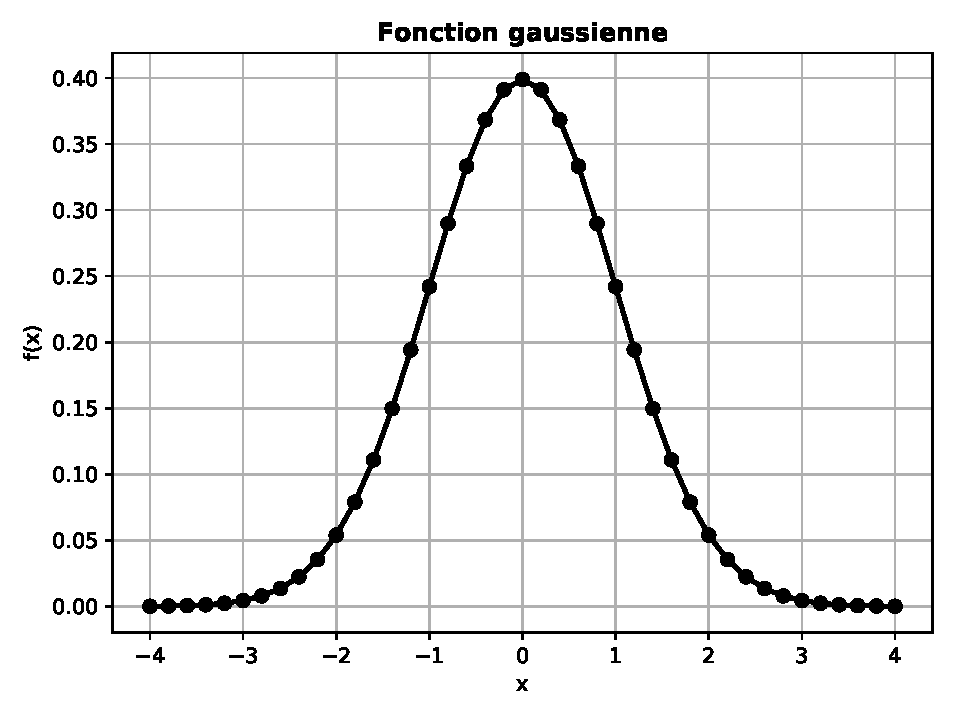
\includegraphics[width=0.5\linewidth]{scripts/gauss.pdf}}

\vspace{6mm}



% --- end hint in exercise ---


% --- begin solution of exercise ---
\paragraph{Solution.}
Le graphique sera généré en implémentant le code suivant:
\begin{cod}{cbg_gray}\begin{minted}[fontsize=\fontsize{9pt}{9pt},linenos=false,mathescape,baselinestretch=1.0,fontfamily=tt,xleftmargin=2mm]{python}
import matplotlib.pyplot as plt

plt.plot(x, f(x), 'ko-',lw=2)
plt.title("Fonction gaussienne", fontweight='bold')
plt.xlabel("x")
plt.ylabel("f(x)")
plt.grid()
plt.tight_layout()
plt.savefig("gauss.png"); plt.savefig("gauss.pdf")

\end{minted}
\end{cod}
\noindent

% --- end solution of exercise ---

\end{doconceexercise}
% --- end exercise ---


% !split


% --- begin exercise ---
\begin{doconceexercise}
\refstepcounter{doconceexercisecounter}

\exercisesection{Exercise \thedoconceexercisecounter: Tracer la viscosité de l'eau (5 points)}


La viscosité de l'eau, $\mu$, varie avec la température $T$ (en Kelvin) selon la formule:
\begin{equation}
\mu (T) = A\cdot 10^{B/(T-C)}
\end{equation}
où $A=2.414\cdot 10^{-5}\hbox{ Pa s}$, $B=247.8 \ K$ et $C = 140 \ K$.


\subex{a)}
Définir la fonction \texttt{mu(T, A, B, C)} qui renvoie la valeur de la viscosité $\mu$ pour chaque valeur donnée de la température $T$.


% --- begin solution of exercise ---
\paragraph{Solution.}
La fonction \texttt{mu(T, A, B, C)} est définie comme suivant:
\begin{cod}{cbg_gray}\begin{minted}[fontsize=\fontsize{9pt}{9pt},linenos=false,mathescape,baselinestretch=1.0,fontfamily=tt,xleftmargin=2mm]{python}
def mu(T, A, B, C):
    return A*10**(B/(T-C))
\end{minted}
\end{cod}
\noindent

% --- end solution of exercise ---

\subex{b)}
Tracer $\mu (T)$ pour 20 valeurs de $T$ entre 0 et 100 degrés Celsius. Marquer l'axe des $x$ avec "Température (degrés Celsius)", l'axe des $y$ avec "viscosité (Pa~s)" et le titre "Évolution de la viscosité de l'eau avec la température". \textbf{Notez que $T$ dans la formule de $\mu$ doit être en Kelvin}.

% --- begin hint in exercise ---

\paragraph{Indication.}
\begin{itemize}
\item On vous donne: 0 deg C = 273 deg K

\item La sortie du programme devrait ressembler à la figure ci-dessous.
\end{itemize}

\noindent
\vspace{6mm}

% inline figure
\centerline{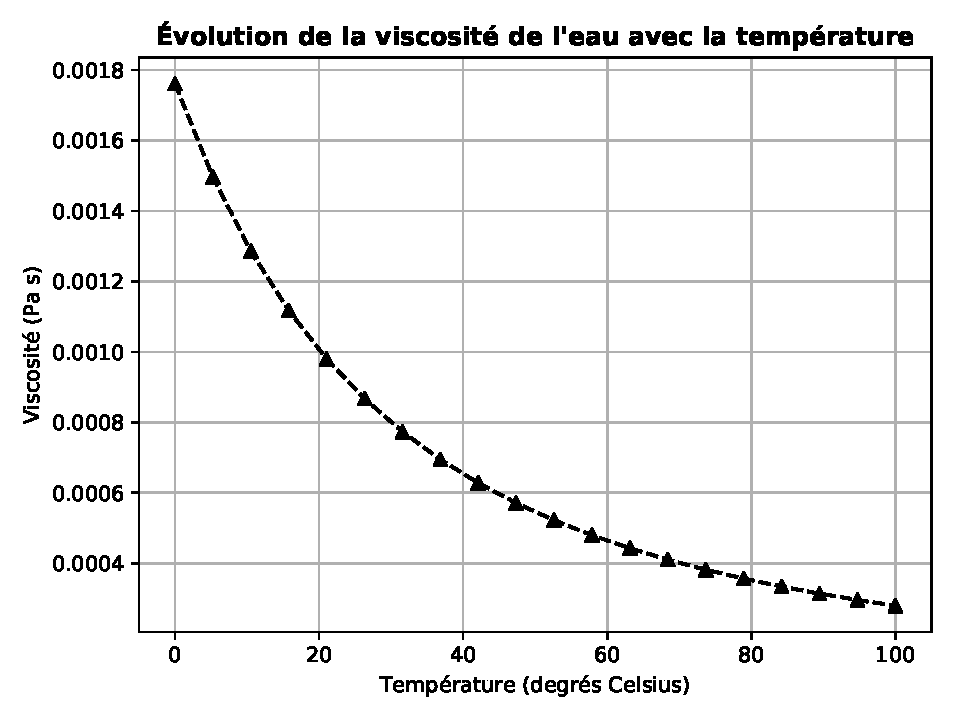
\includegraphics[width=0.5\linewidth]{scripts/viscosity.pdf}}

\vspace{6mm}



% --- end hint in exercise ---


% --- begin solution of exercise ---
\paragraph{Solution.}
Le code qui trace la viscosité de l'eau en fonction de la température est comme suivant:
\begin{cod}{cbg_gray}\begin{minted}[fontsize=\fontsize{9pt}{9pt},linenos=false,mathescape,baselinestretch=1.0,fontfamily=tt,xleftmargin=2mm]{python}
import matplotlib.pyplot as plt
import numpy as np
# 0 deg C = 273 deg K
T = np.linspace(0, 100, 20)

plt.plot(T, mu(T+273, A = 2.414e-5, B = 247.8, C = 140), 'k^--')
plt.title("Évolution de la viscosité de l'eau avec la température",
          fontweight='bold')
plt.xlabel("Température (degrés Celsius)")
plt.ylabel("Viscosité (Pa s)")
plt.grid()
plt.savefig("viscosity.png"); plt.savefig("viscosity.pdf")
\end{minted}
\end{cod}
\noindent

% --- end solution of exercise ---

\end{doconceexercise}
% --- end exercise ---


% ------------------- end of main content ---------------

% #ifdef PREAMBLE
\end{document}
% #endif

